\documentclass[inzynier,druk]{helpers/dyplom}
\usepackage[utf8]{inputenc}
\usepackage{hyperref}
%%
\usepackage[toc]{appendix}
\renewcommand{\appendixtocname}{Dodatki}
\renewcommand{\appendixpagename}{Dodatki}

% pakiet do składu listingów w razie potrzeby można odblokować możliwość numerowania linii lub zmienić wielkość czcionki w listingu
\usepackage{minted}
\setminted{breaklines,
frame=lines,
framesep=5mm,
baselinestretch=1.1,
fontsize=\small,
%linenos
}

% nowe otoczenie do składania listingów
\usepackage{float}
\newfloat{listing}{htp}{lop}
\floatname{listing}{Listing}
\usepackage{chngcntr}
\counterwithin{listing}{chapter}

% patch wyrównujący spis listingów do lewego marginesu 
%https://tex.stackexchange.com/questions/58469/why-are-listof-and-listoffigures-styled-differently
\makeatletter
\renewcommand*{\listof}[2]{%
  \@ifundefined{ext@#1}{\float@error{#1}}{%
    \expandafter\let\csname l@#1\endcsname \l@figure  % <- use layout of figure
    \float@listhead{#2}%
    \begingroup
      \setlength\parskip{0pt plus 1pt}%               % <- or drop this line completely
      \@starttoc{\@nameuse{ext@#1}}%
    \endgroup}}
\makeatother

\usepackage{url}
\usepackage{lipsum}

% Dane o pracy
\author{<Imię i Nazwisko Autora>}
\title{<Tytuł pracy>}
\titlen{<Angielskie tłumaczenie tytułu>}
\promotor{<Tytuł naukowy Imię i Nazwisko Promotora>}
%\konsultant{dr hab. inż. Kazimerz Kabacki}
\wydzial{Wydział Informatyki i Zarządzania}
\kierunek{Informatyka}
\krotkiestreszczenie{W pracy przedstawiono projekt aplikacji służącej do komunikacji z kosmitami, wykorzystujący framework SpaceDirect i bazę danych NoMySQL}
\slowakluczowe{kosmici, NoMySQL, SpaceDirect, aplikacja mobilna}

\begin{document}

\maketitle

\tableofcontents

\listoffigures

\listof{listing}{Spis listingów}

\listoftables

% --- Strona ze streszczeniem i abstraktem ------------------------------------------------------------------
\chapter*{Streszczenie} % po polsku
% Wprowadzenie
Celem pracy było opracowanie aplikacji służącej do komunikacji z kosmitami. Dostępne na rynku aplikacj e nie satysfakcjonowały autorki ze względu na brak istotnych funkcji takich jak obsługa przez telefon z systemem Android.
% Sposób rozwiązania problemu
W ramach pracy przygotowano aplikację komunikacyjną wykorzystującą framework SpaceDirect, przechowującą dane kontaktów w bazie danych MyNoSQL oraz udostępniającą swoje funkcje przez interfejs REST API.
% Dodatkowe informacji o pracy
Oprócz projektu aplikacji praca zawiera wyniki testów jednostkowych oraz testów użyteczności przeprowadzonych przez krewnych i znajomych królika.
% Podsumowanie
Przygotowana w ramach projektu inżynierskiego praca może zostać wykorzystana przez wszystkie osoby zainteresowane kontaktami z cywilizacjami pozaziemskimi.


% Kilka sztuczek, żeby:
% - Abstract pojawił się na tej samej stronie co Streszczenie
% - Abstract nie pojawił się w spisie treści
\addtocontents{toc}{\protect\setcounter{tocdepth}{-1}}
\begingroup
\renewcommand{\cleardoublepage}{}
\renewcommand{\clearpage}{}
\chapter*{Abstract} % ...i to samo po angielsku
The main goal of this thesis was development of\dots (\textit{please translate remaining part of Streszczenie into English}).


\endgroup
\addtocontents{toc}{\protect\setcounter{tocdepth}{2}}

% --- Koniec strony ze streszczeniem i abstraktem -----------------------------------------------------------


% Rozdział dołączony z zewnątrz
\input{wstep}

\input{rozdzial1}

\chapter{Ala ma kota}

ĄĆĘŁŃÓŚŹŻ ąćęłńóśźż\footnote{Przykład użycia polskich znaków diakrytycznych oraz przypisu w miejscu}. \lipsum[1]

\section{Odniesienie do pozycji z literatury (strona WWW)}

% Odniesienie do rysunku i cytowanie dokumentu. Dokumenty są definiowane w pliku literatura.bib
Reszta dokumentacji znajduje się w \cite{docker_compose_reference}. \lipsum[3]

\section{Odniesienie do książki}

Jak pisze Harel w \cite{harel_rzecz_2008}: \lipsum[7]

\section{Rysunek}

% Rysunek
\begin{figure}
\centering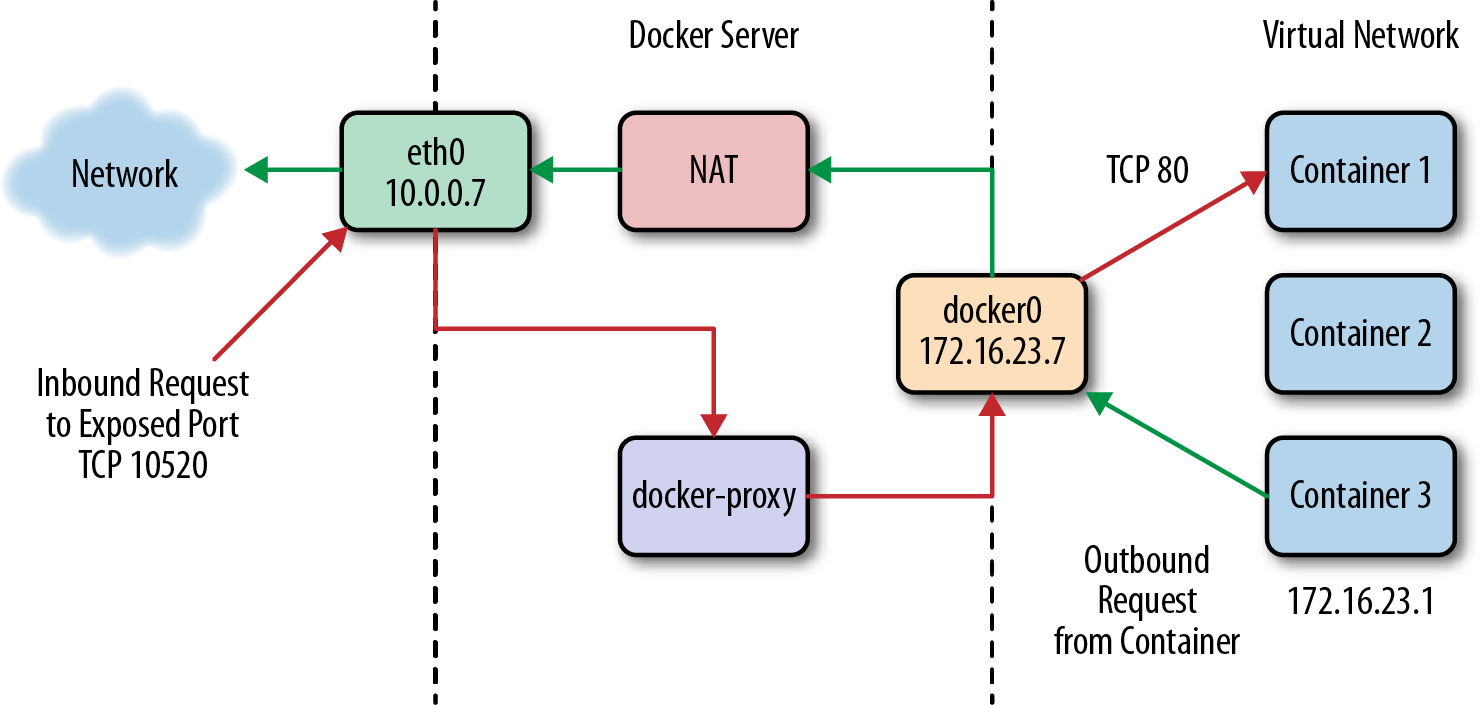
\includegraphics[width=.6\textwidth]{images/swarm-network.png}
\caption{Docker ma sieć \cite{docker_compose_reference}.}  \label{rys:network}% Źródło rysunku i etykieta przez którą odwołujemy się do rysunku.
\end{figure}

Jak widać na rys. \ref{rys:network} Docker ma wewnętrzną sieć. \lipsum[1]


\subsection{Rysunek z kotem}

Jak widać na rys.\ref{rysunek:kot} Ala ma kota. \lipsum[9-10] 

\begin{figure}
\centering
\includegraphics[width=.4\textwidth]{img/kotek}
\caption{Ala ma kota (opr.wł).}\label{rysunek:kot}
\end{figure}

\subsection{Tabela}

Co uwzględniono w tabeli \ref{tabela:coktoma}. \lipsum[13-15] 

% Tabela. Nazwa tabeli u góry.
\begin{table}
\centering\caption{Co kto ma \cite{harel_rzecz_2008} (patrz też dodatek~\ref{Dod1}) \label{tabela:coktoma}}
\begin{tabular}{|l|l|l|}% wyrównanie kolumn tabeli -> l c r - do lewej, środka, do prawej
\hline
Ala & ma & kota \\
\hline
Ola & ma & psa \\
\hline
Ula & ma & małpę\\
\hline
\end{tabular}
\end{table}

\lipsum[19-20] Warto wspomnieć, że w \cite{aizawa_groundwater_2009} rzecz przedstawiona jest zupełnie inaczej. Poniższy wzór:

\begin{equation}
\sum_{i=1}^{\infty}a_i
\label{eq:mojWzor}
\end{equation}

Wzór \ref{eq:mojWzor} wskazuje że dowód podany w \cite{kaleta_experimental_2005} może zostać podważony. \lipsum[9]

\section{Listing}

% lub {java} albo {bash} albo {text}
\begin{listing}
\begin{minted}{c} 
int main()
{
   int a=2*3;
   printf("**Ala ma kota\n**");
   while(!I2C_CheckEvent(I2C1, I2C_EVENT_MASTER_MODE_SELECT)); /* EV5 */
   return 0;
}
\end{minted}
\caption{Przykładowy algorytm w języku C (opr. wł.)} \label{listing:moj}
\end{listing}

W moim kodzie \ref{listing:moj} zrobiłem coś wspaniałego. \lipsum[4]



\chapter*{Zakończenie}

W pracy udało mi się dużo zrobić. \lipsum[17]

Mnóstwo innych rzeczy da się poprawić i rozwinąć. \lipsum[23]

\appendixpage
\appendix
%\addappheadtotoc

\chapter{To powinien być dodatek}\label{Dod1}

\lipsum[9-11]

% W pracy pojawią się tylko prace naprawdę cytowane.
% \nocite{*}

\bibliography{literatura}
\bibliographystyle{dyplom}

\end{document}
